%!TEX program = xelatex
%Template created by: Maciej Byczko
\documentclass[a4paper,12pt]{extarticle}  %typ dokumentu

\usepackage{geometry} %poprawienie marginesów
\usepackage{polski} %polskie znaki
\usepackage{graphicx} %grafiki
\usepackage{float} %poprawienie pozycji
\usepackage{fancyhdr} % header i footer
\usepackage{listings}
\usepackage{xcolor}
\usepackage{hyperref}
\graphicspath{{pictures/}}
\geometry{margin=0.7in}
\pagestyle{fancy}
\cfoot{Strona \thepage}
\rhead{Strona \thepage}
\lhead{\typdoc}
\setlength{\headheight}{15pt}

\title{\tytul \\ \small{\opis}}
\author{\tworcy}
\date{\data}

%-----------------------SEKCJA DANYCH----------------------------------
\def\tytul{Raspberry Pi} %<<< tytuł ćwiczenia
\def\nrcw{laboratoria 17} %<<< numer ćwiczenia
\def\data{\today} %<< data wykonania
\def\prowadzacy{Dr inż. Dominik Żelazny} %<<<prowadzący
\def\nrgrupy{D} %<<<numer grupy
\def\tworcy{Baraniecki Karol\\Byczko Maciej} %<<< autorzy
\def\zajinfo{PT 16:30 TP} %<<< informacje dotyczące zajęć
\def\typdoc{Sprawozdanie} %<<< typ dokumentu tj Sprawozdanie, zadania itp. {Matematyka dyskretna/Sprawozdanie z Miernictwa}
\def\opis{} %<<< opis który będzie umieszczony pod tytułem w Maketitle
%----------------------------------------------------------------------

\definecolor{backcolour}{rgb}{0.95,0.95,0.92}
\definecolor{AO}{rgb}{0,0.5,0}
\definecolor{ZeroBlue}{rgb}{0,0.28,0.73}
\definecolor{DarkRed}{rgb}{0.85,0.16,0.16}

%Ustawienie paczki hyperref
\hypersetup{
     colorlinks = true,
     citecolor=black,
     filecolor=black,
     linkcolor=blue,
     urlcolor=blue
}

\lstset{
basicstyle=\footnotesize,
breaklines=true,
language=Python,
numbers=left,
tabsize=2,
numberstyle=\tiny,
backgroundcolor=\color{backcolour},
breakatwhitespace=false,
showspaces=false,                
showstringspaces=false,
showtabs=false,
commentstyle=\color{gray},
keywordstyle=\color{ZeroBlue},
keepspaces=true,
% keywordstyle={[2]\color{DarkRed}},
% keywordstyle={[3]\color{ZeroBlue}},
}

\begin{document}
%-------------------------------------TABELA-DANYCH--------------------------------------------------
\begin{table}[H]
	\centering
	\resizebox{\textwidth}{!}{
		\begin{tabular}{|c|c|c|}\hline
			\begin{tabular}[c]{@{}c@{}}                     \tworcy     \end{tabular} &
			\begin{tabular}[c]{@{}c@{}}Prowadzący:\\        \prowadzacy \end{tabular} &
			\begin{tabular}[c]{@{}c@{}}Numer ćwiczenia\\    \nrcw       \end{tabular}          \\ \hline
			\begin{tabular}[c]{@{}c@{}}                     \zajinfo    \end{tabular} &
			\begin{tabular}[c]{@{}c@{}}Temat ćwiczenia:\\   \tytul      \end{tabular} & Ocena: \\ \hline
			\begin{tabular}[c]{@{}c@{}}Grupa:\\          \nrgrupy    \end{tabular}    &
			\begin{tabular}[c]{@{}c@{}}Data wykonania:\\    \data       \end{tabular} &        \\ \hline
		\end{tabular}}
\end{table}
%----------------------------------------------------------------------------------------------------
\section{Zagadnienia do opracowania}
\begin{enumerate}
	\item Urządzenia RPI (wersja 4)
	      \begin{itemize}
		      \item \href{https://www.raspberrypi.org/}{Raspberry Pi} - platforma komputerowa stworzona przez Raspberry Pi Foundation. Urządzenie składa się z pojedynczego obwodu drukowanego i zostało wymyślone, by wspierać naukę podstaw informatyki.
		      \item interfejs GPIO (numeracja pinów) - Wejście-wyjście ogólnego przeznaczenia, GPIO (od ang. general-purpose input/output), pin interfejsu do komunikacji między elementami systemu komputerowego (na przykład między mikroprocesorem a urządzeniami peryferyjnymi).
	      \end{itemize}
	\item Środowisko programistyczne
	      \begin{itemize}
		      \item zasady pracy z systemem Linux - NIE WYKONUJ KOMENDY \emph{rm -rf /*}
		      \item interfejs wiring Pi - biblioteka do obsługi GPIO
		      \item język python, zasady instalacji pakietów (pip) - język programowania wysokiego poziomu ogólnego przeznaczenia, o rozbudowanym pakiecie bibliotek standardowych, którego ideą przewodnią jest czytelność i klarowność kodu źródłowego. Jego składnia cechuje się przejrzystością i zwięzłością.
		      \item sterowanie sygnałami wejściowymi/wyjściowymi
		            \begin{itemize}
			            \item RPi.GPIO - Raspberry Pi GPIO - Moduł do sterowania diodami
		            \end{itemize}
	      \end{itemize}
	\item Zestaw prototypowy
	      \begin{itemize}
		      \item picoboard - Zestaw prototypowy dla Raspberry Pi
		      \item zasady podłączania diody - diodę należy podłączyć przez opornik aby się nie spalił pin w Raspberry.
		      \item interfejs 1-wire i czujnik temperatury DS18B20
	      \end{itemize}
\end{enumerate}
\section{Zadania do wykonania}
\begin{enumerate}
	\item Testy urządzenia
	      \begin{itemize}
		      \item podłączyć urządzenia: zasilanie + kabel ethernet
		            %todo wstawić zdjęcie układu
		            \begin{figure}[H]
			            \centering
			            \resizebox*{\textwidth}{!}{
				            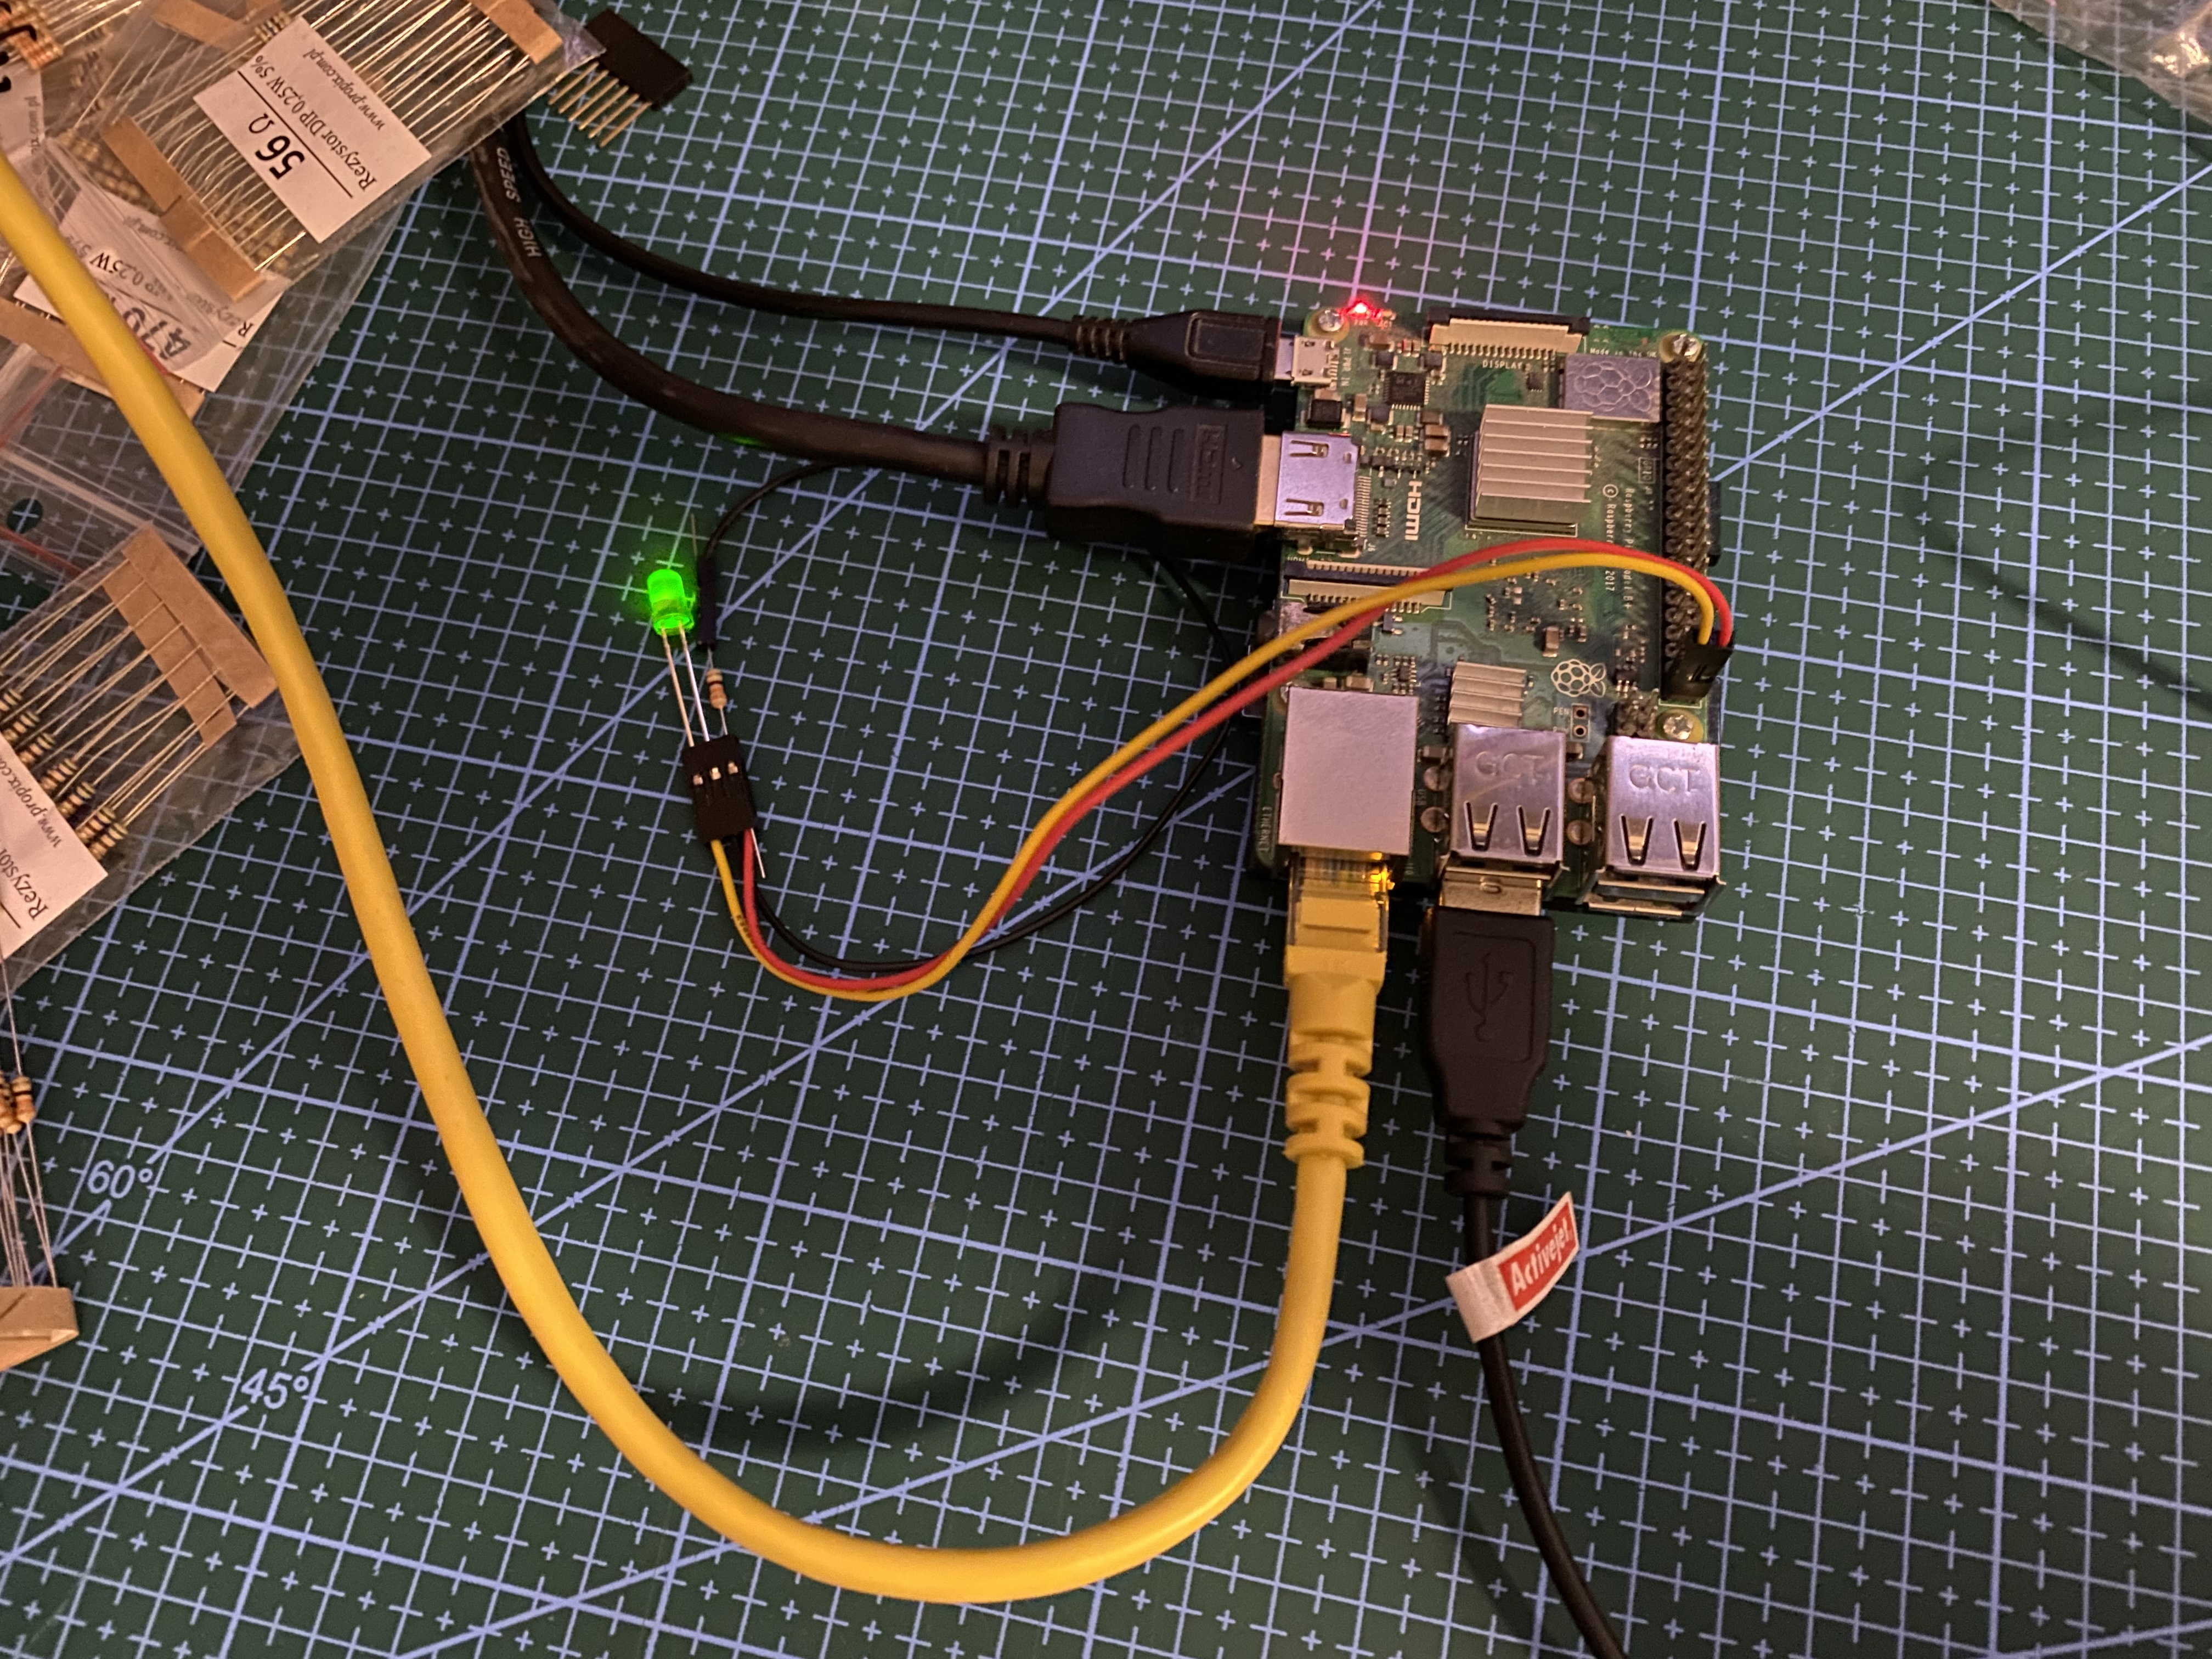
\includegraphics{fizyczny.JPG}
			            }
		            \end{figure}
		      \item określenie adresu IP (podłączyć monitor, adres IP podany będzie na ekranie (ew. komenda ifconfig))
		            % todo wstawić screenshot 
		            \begin{figure}[H]
			            \centering
			            \resizebox*{\textwidth}{!}{
				            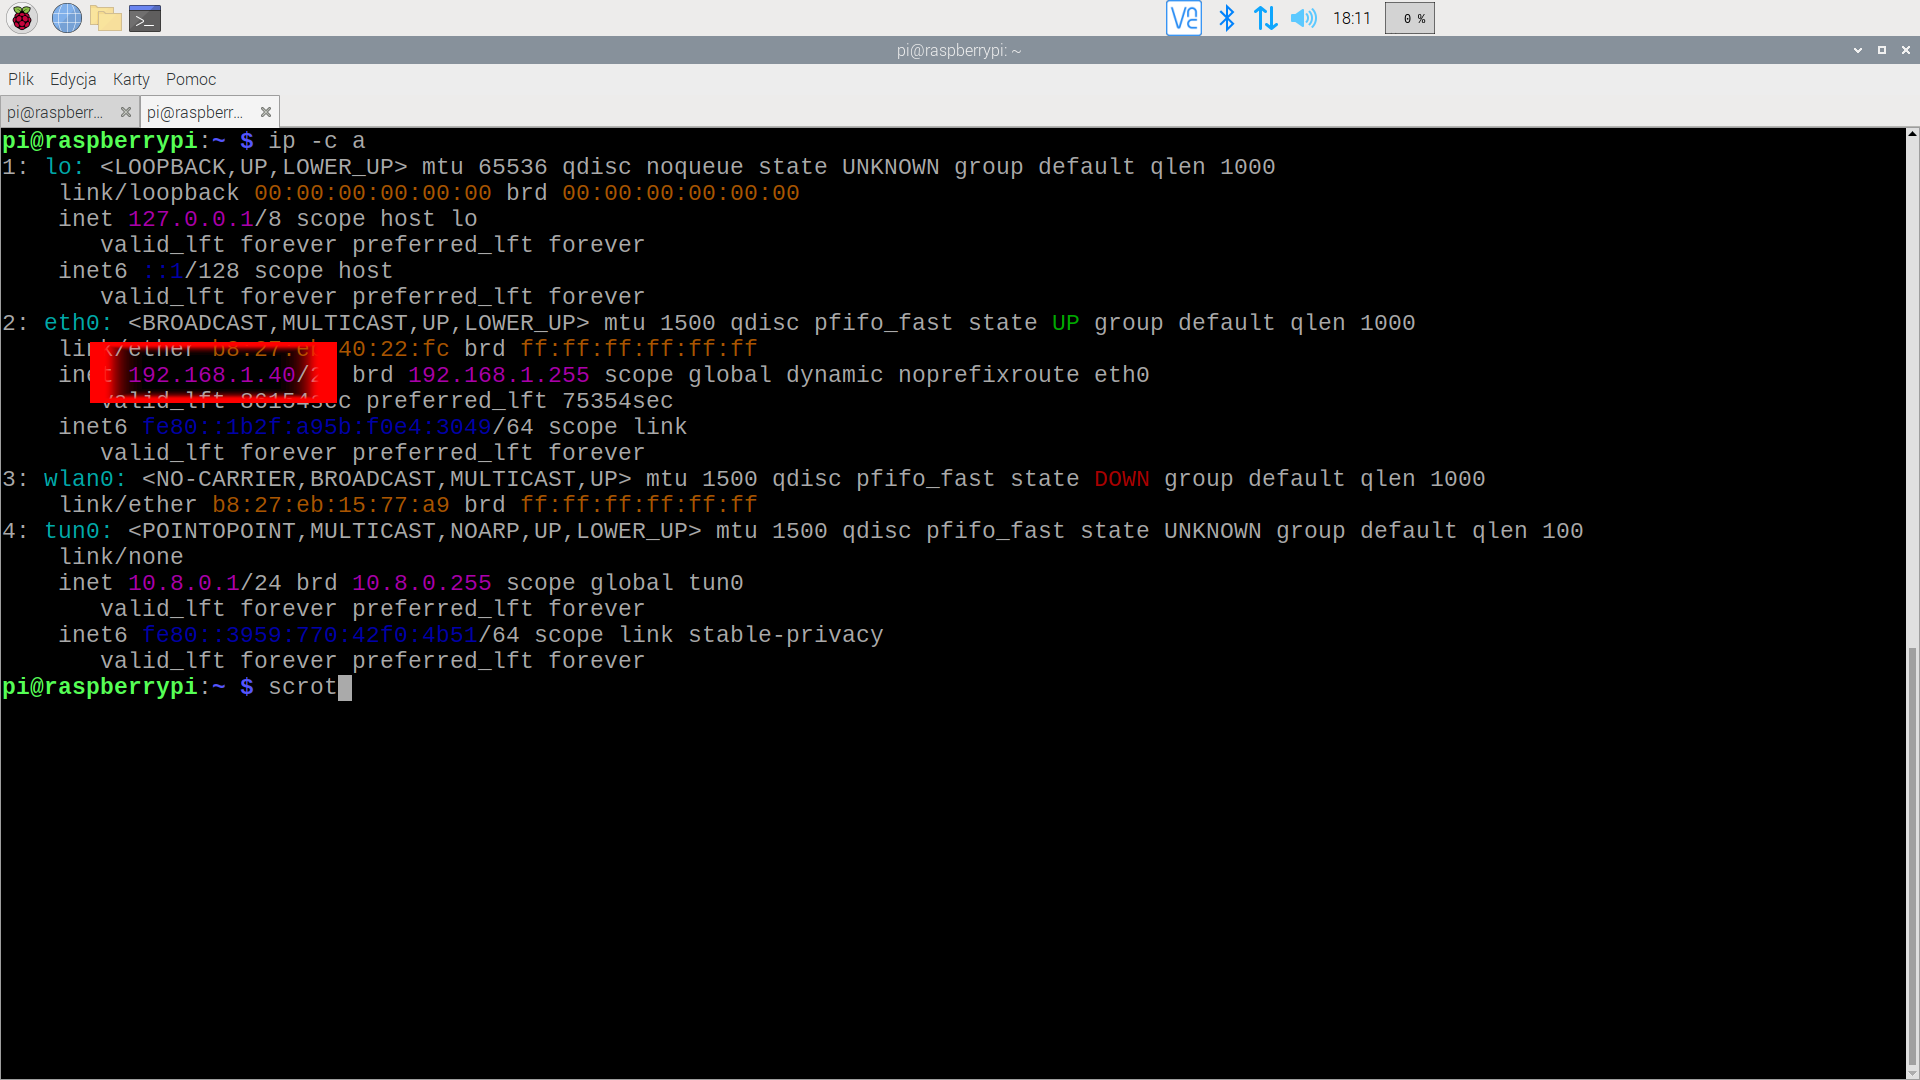
\includegraphics{ip_address.png}
			            }
		            \end{figure}
		      \item zalogowanie na konsole via putty (proszę nie zmieniać hasła) (dostęp: pi, raspberry)\\
		            Zalogowaliśmy się za pomocą OpenSSH w terminalu, gdyż PuTTY wymaga dodatkowych instalacji a robi to samo.
		            \begin{figure}[H]
			            \centering
			            \resizebox*{\textwidth}{!}{
				            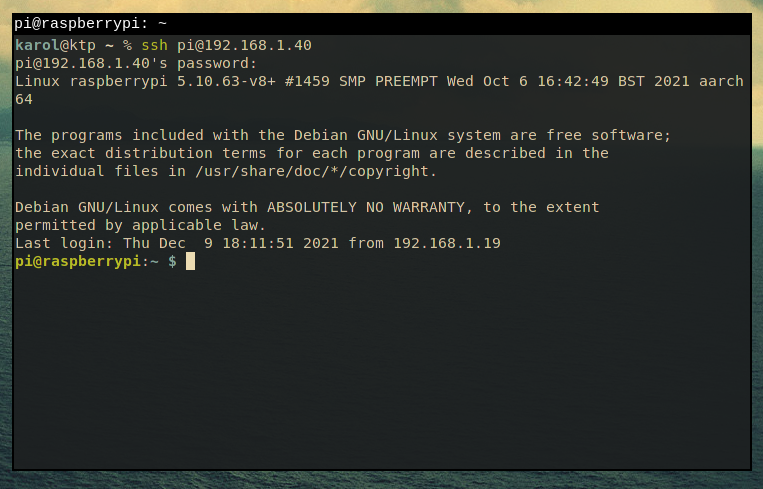
\includegraphics{raspi_ssh.png}
			            }
		            \end{figure}
	      \end{itemize}

	\item Sterowanie diodą
	      \begin{itemize}
		      \item podłączenie diody i rezystora do RPi (przed podłączaniem zasilania proszę poprosić prowadzącego o sprawdzenie połączeń)
		            \begin{figure}[H]
			            \centering
			            \resizebox*{\textwidth}{!}{
				            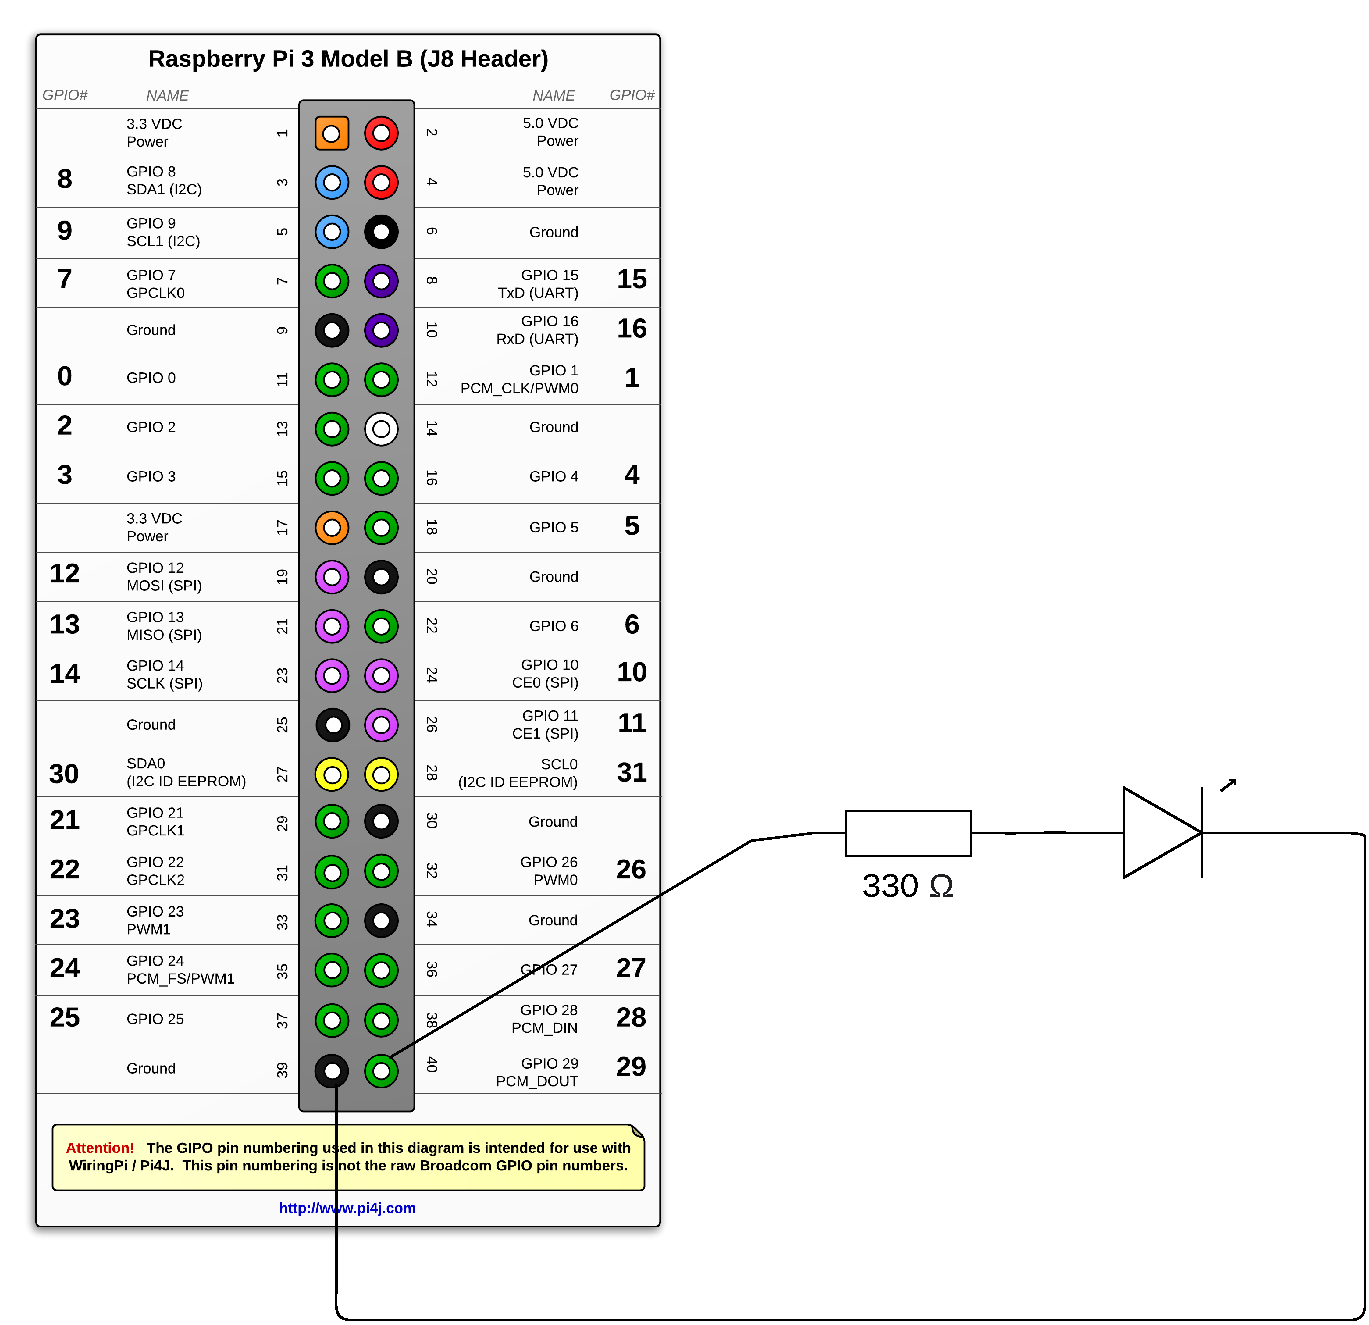
\includegraphics{diagram_polaczenia.pdf}
			            }
		            \end{figure}
		      \item sterowanie z poziomu programu gpio
		            \begin{lstlisting}[language = Bash]
gpio -1 mode 40 out # ustawienie pinu jako wyjscie
gpio -1 write 40 1 # wlaczenie diody
gpio -1 write 40 0 # wylaczenie diody
gpio -1 blink 40 # wlaczenie trybu migania diody
\end{lstlisting}
		      \item program w pythonie
		            \begin{lstlisting}[language = Python]
import time
import RPi.GPIO as GPIO

GPIO.setmode(GPIO.BOARD)
PIN = 40

GPIO.setup(PIN, GPIO.OUT)
while True:
    time.sleep(0.1)
    GPIO.output(PIN, 0)
    time.sleep(0.1)
    GPIO.output(PIN, 1)
        \end{lstlisting}
	      \end{itemize}
\end{enumerate}

\section{Wnioski}
\href{https://s3.baraniecki.eu/rasp_led.webm}{Film Video z działającym układem}\\
Zadanie było w miarę proste, pogubiliśmy się przy numeracji pinów a poza tym wszystko potoczyło się bez większych problemów.

\end{document}